\mysubsection{Linda Schey}{Multimonitor Support}

Schon zu Beginn des Projektes wurde versucht, eine möglichst große Projektionsfläche zu erreichen. In Ermangelung eines leistungsstarken Beamers, wurde auf drei Beamer zurückgegriffen, die dann nebeneinander je ein Drittel der Applikation darstellen sollten. Um dies zu realisieren, musste aber das zu projizierende Bild in drei einzelne Bilder geteilt werden. Da die Beamer aber, um ein größeres Bild zu erzielen, nicht nebeneinander, sondern übereinander aufgebaut werden sollten, mussten die erhaltenen Bilder jeweils um 90° gedreht werden. Dafür wurde in Unity eine neue Kamera erstellt, die die Szene als \emph{RenderTexture} aufnahm. Diese RenderTexture wurde dann in drei einzelne Texturen getrennt, jede Textur um 90° gedreht und anschließend nebeneinander auf der GUI dargestellt. Dies war bereits fertig in BlinkenTiles implementiert.

\begin{figure}[htbp]
	\centering
		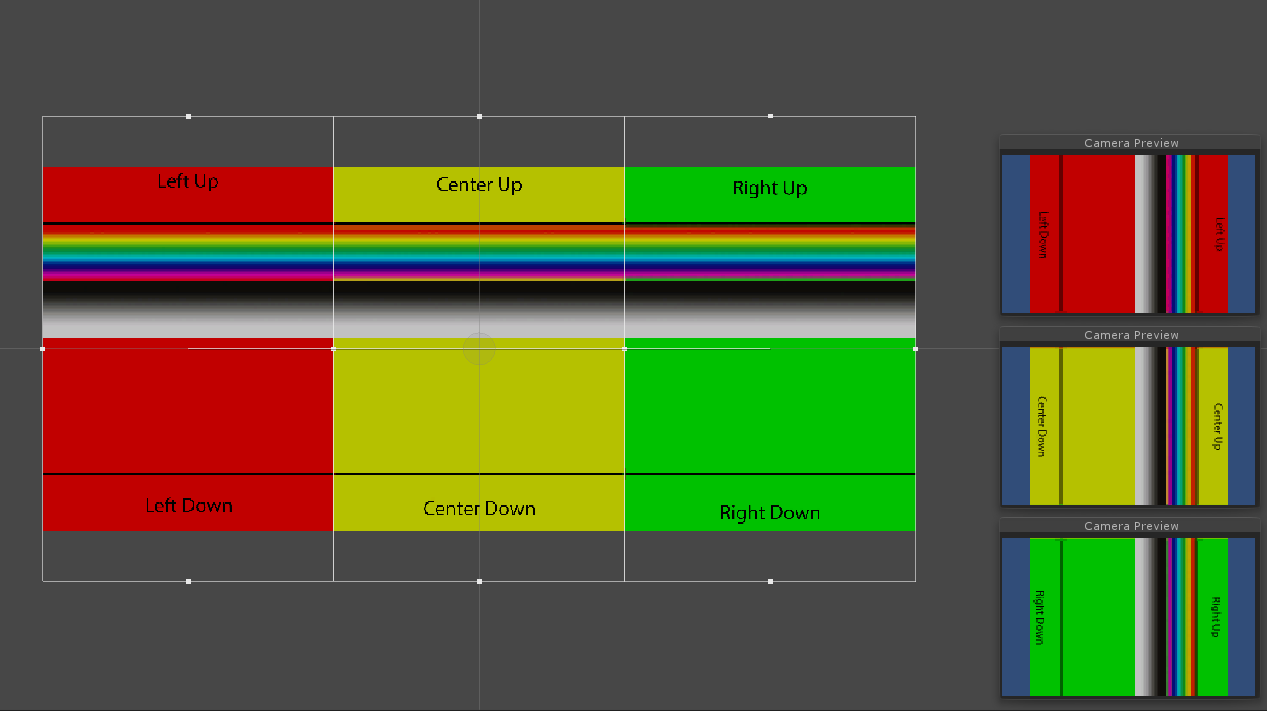
\includegraphics[width=0.9\textwidth]{images/RenderTextureBeispielSzene.PNG}
	\caption{Aufbau der Szene in Unity mit drei RenderTexture-Ausschnitten am Beispiel eines Testobjektes}
	\label{fig:RenderTextureBeispielSzene}
\end{figure}

\begin{figure}[htbp]
	\centering
		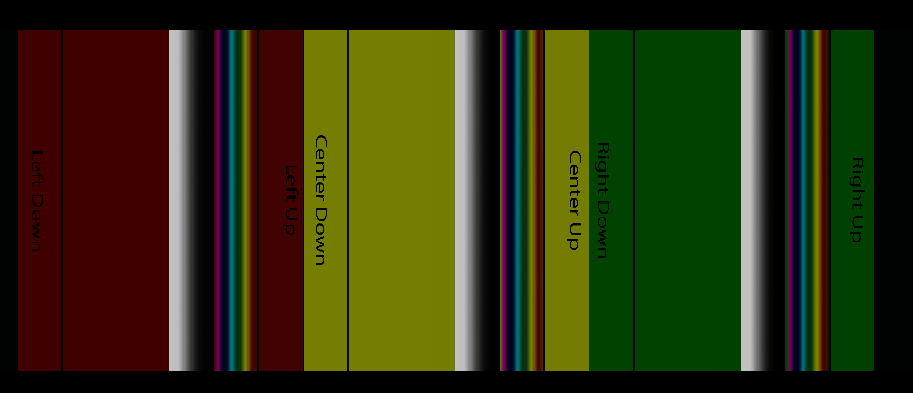
\includegraphics[width=0.9\textwidth]{images/RenderTexturesAlsGui.PNG}
	\caption{RenderTextures nebeneinander auf die GUI gerendert}
	\label{fig:RenderTexturesAlsGui}
\end{figure}

Ein anderer Ansatz war drei um 90° gedrehte Kameras in die Szene zu integreren die jeweils ein Drittel des Spielfeldes filmten. Hier wurde zunächst mit einem Beispielobjekt gearbeitet, das ein Material zugewiesen bekam. Dies vereinfachte die Entwicklung, da so erkannt werden konnte, ob die Kameras richtig ausgerichtet waren und dann auch entsprechend richtig auf die GUI gerendert wurden. Die drei Kameras mussten jedoch von Hand auf die Szene eingestellt werden, so dass es auch hier wieder zu Ungenauigkeiten hätte kommen können. Andererseits wäre man hier flexibler beim Ausrichten der Szene auf die drei Beamer gewesen, indem man zum Beispiel die Übergänge zwischen den drei Texturen jeweils so hätte platzieren können, dass sie auf einem Spalt zwischen den Feldern des Spielfeldes gelegen wären. Auch dieser Ansatz wurde umgesetzt und hat funktioniert allerdings auch mit kleinen Ungenauigkeiten.

Beide Ansätze waren jedoch nicht zu 100 Prozent exakt, was das Aufteilten der Szene in drei Teil-Texturen betraf. Außerdem standen keine drei identischen Beamer zur Verfügung, sodass es unter den einzelnen Beamern Unterschiede bei der Lichtintensität gab. Da anstatt der Lösung mit den drei Beamern letztlich doch noch ein geeignetes Gerät gefunden wurde, das alleine die gewünschte Projektionsfläche erbrachte, wurde die Idee mit den drei Beamern sowie die bisherige Implementierung dafür verworfen und ist im finalen Stand des Projektes nicht mehr enthalten.